\documentclass[a4paper,12pt]{article}
\usepackage[brazil]{babel}
\usepackage[utf8]{inputenc}
\usepackage{indentfirst}
\usepackage{amsmath}
\usepackage{amsthm}
\usepackage{graphicx}
\usepackage{float}
\usepackage{array}
\usepackage[font=footnotesize,labelfont=bf]{caption}
\usepackage{geometry}
\usepackage{listings}
\usepackage{subcaption}
\usepackage{xcolor}
\usepackage[skins,xparse,breakable]{tcolorbox}
\usepackage{longtable}
\usepackage{minted}
\usepackage{lastpage}
\usepackage{graphicx}
\usepackage{dirtree}
\usepackage{mdframed}
\usepackage{enumitem}
\usepackage{geometry}
\usepackage{titlesec}
\usepackage{fancyhdr}
\usepackage{setspace}
\usepackage[colorlinks=true, allcolors=black]{hyperref}

% Configurações de margens e espaçamento
\geometry{a4paper, left=3cm, right=2cm, top=3cm, bottom=2cm}
\setlength{\parindent}{1.25cm}
\onehalfspacing

% Configurações de títulos
\titleformat{\section}{\normalfont\large\bfseries}{\thesection}{1em}{}
\titleformat{\subsection}{\normalfont\bfseries}{\thesubsection}{1em}{}
\titleformat{\subsubsection}{\normalfont\itshape}{\thesubsubsection}{1em}{}

% Configurações de listagens
\renewcommand{\listingscaption}{Código}
\newenvironment{code}{\captionsetup{type=listing}}{}

% Configurações de cabeçalho e rodapé
\pagestyle{fancy}
\fancyhf{}
\fancyhead[L]{\footnotesize{Tonhão Autopeças - Proposta de Projeto TP1 - Grupo 08}}
\fancyhead[R]{\footnotesize{\thepage\ de \pageref{LastPage}}}
\fancyfoot[C]{\footnotesize{Relatório de implementação do sistema do Tonhão Autopeças}}

% Definindo cores personalizadas
\definecolor{roxo}{RGB}{171, 71, 188} % Roxo
\definecolor{verde}{RGB}{0, 128, 0} % Verde
\definecolor{cinza_claro}{RGB}{240, 240, 240} % Cinza claro
\definecolor{verde_claro}{RGB}{124, 200, 66} % Verde claro
\definecolor{vermelho}{RGB}{239, 83, 80} % Vermelho
\definecolor{verde_marinho}{RGB}{0, 150, 136} % Verde Marinho

\begin{document}

% Capa
\begin{titlepage}
    \begin{center}
        \vspace*{2cm}
        {\Large \textbf{Universidade de Brasília (UnB)}} \\
        {\Large \textbf{Departamento de Ciência da Computação}} \\
        \vspace{3cm}
        {\Huge \textbf{Tonhão Autopeças}} \\
        \vspace{1cm}
        {\Large \textbf{Proposta de Projeto TP1}} \\
        \vspace{2cm}
        {\Large \textbf{Grupo 08}} \\
        \vspace{1cm}
        {\Large \textbf{Nirva Neves de Macedo, 232009585}} \\
        {\Large \textbf{Henrique Morcelles Salum, 232003008}} \\
        {\Large \textbf{Dérick Daniel Silva de Andrade, 231003522}} \\
        \vspace{2cm}
        {\Large \textbf{Brasília, 21 de outubro de 2024}}
    \end{center}
\end{titlepage}

% Sumário
\newpage
\tableofcontents
\newpage

% Introdução
\section{Descrição do Problema}
\paragraph{}
Oficinas mecânicas são essenciais para a manutenção da infraestrutura centrada em carros no Brasil. Infelizmente, são normalmente conhecidas por suas baixas confiabilidades e desorganização, especialmente quando estão afastadas de polos urbanos.

\paragraph{}
Visando uma solução moderna e simples para essas instituições, propomos um software de gerenciamento baseado em classes, com o objetivo de fornecer uma interface objetiva para gerenciar os seguintes elementos:

\begin{itemize}[noitemsep]
    \item Clientes
    \item Carros
    \item Estoque de peças
    \item Ordens de serviço
\end{itemize}

\paragraph{}
O sistema atribui as ordens de serviço ao cliente, carro e funcionário respectivos, provendo status de conclusão, status de pagamento e método de pagamento. Ele também gerencia o estoque ao solicitar novas peças e deduzir peças usadas em um serviço. O sistema automatiza a demanda de peças, verificando a disponibilidade no estoque e alocando-as automaticamente ao serviço solicitado.


\subsection{Estrutura do Projeto}
\paragraph{}
A parte relevante da estrutura do projeto foi organizada de acordo com a figura abaixo. É importante pontuar, porém, que alguns diretórios foram omitidos; esses são os criados e administrados pelo \textit{NetBeans} ou utilizados para o versionamento pelo \textit{git}.

\begin{figure}[ht]
    \centering
    \begin{mdframed}[
        linewidth=0pt, % Espessura da borda
        roundcorner=10pt, % Borda arredondada
        backgroundcolor=cinza_claro, % Fundo branco
        innertopmargin=10pt, % Espaçamento interno
        innerbottommargin=10pt,
        innerleftmargin=20pt,
        innerrightmargin=20pt
    ]
    \dirtree{%
    .1 \textcolor{black}{Projeto-Final-TP1}.
    .2 \textcolor{verde}{src}.
    .3 \textcolor{red}{app}.
    .4 \textcolor{vermelho}{model}.
    .5 \textit{classes principais}.
    .4 \textcolor{roxo}{ui}.
    .5 \textit{telas}.
    .4 \textcolor{verde_claro}{utils}.
    .5 \textit{classes auxiliares}.
    .3 \textcolor{yellow}{resources}.
    .4 \textcolor{verde_marinho}{images}.
    .5 \textit{imagens utilizadas}.
    }
    \end{mdframed}
    \caption{Estrutura de diretórios do projeto.}
    \label{fig:estrutura}
\end{figure}
    
% Regras de Negócio
\section{Regras de Negócio}
\begin{itemize}[noitemsep]
    \item Clientes que pagarem em dinheiro ou Pix recebem 5\% de desconto.
    \item A cada R\$2.000,00 pagos, o cliente ganha um check-up completo do veículo e troca de óleo gratuitos.
    \item Funcionalidades de cadastrar, alterar e excluir objetos do programa requerem login de administrador.
\end{itemize}

% Diagrama de Classes
\section{Diagrama de Classes}
\begin{figure}[H]
    \centering
    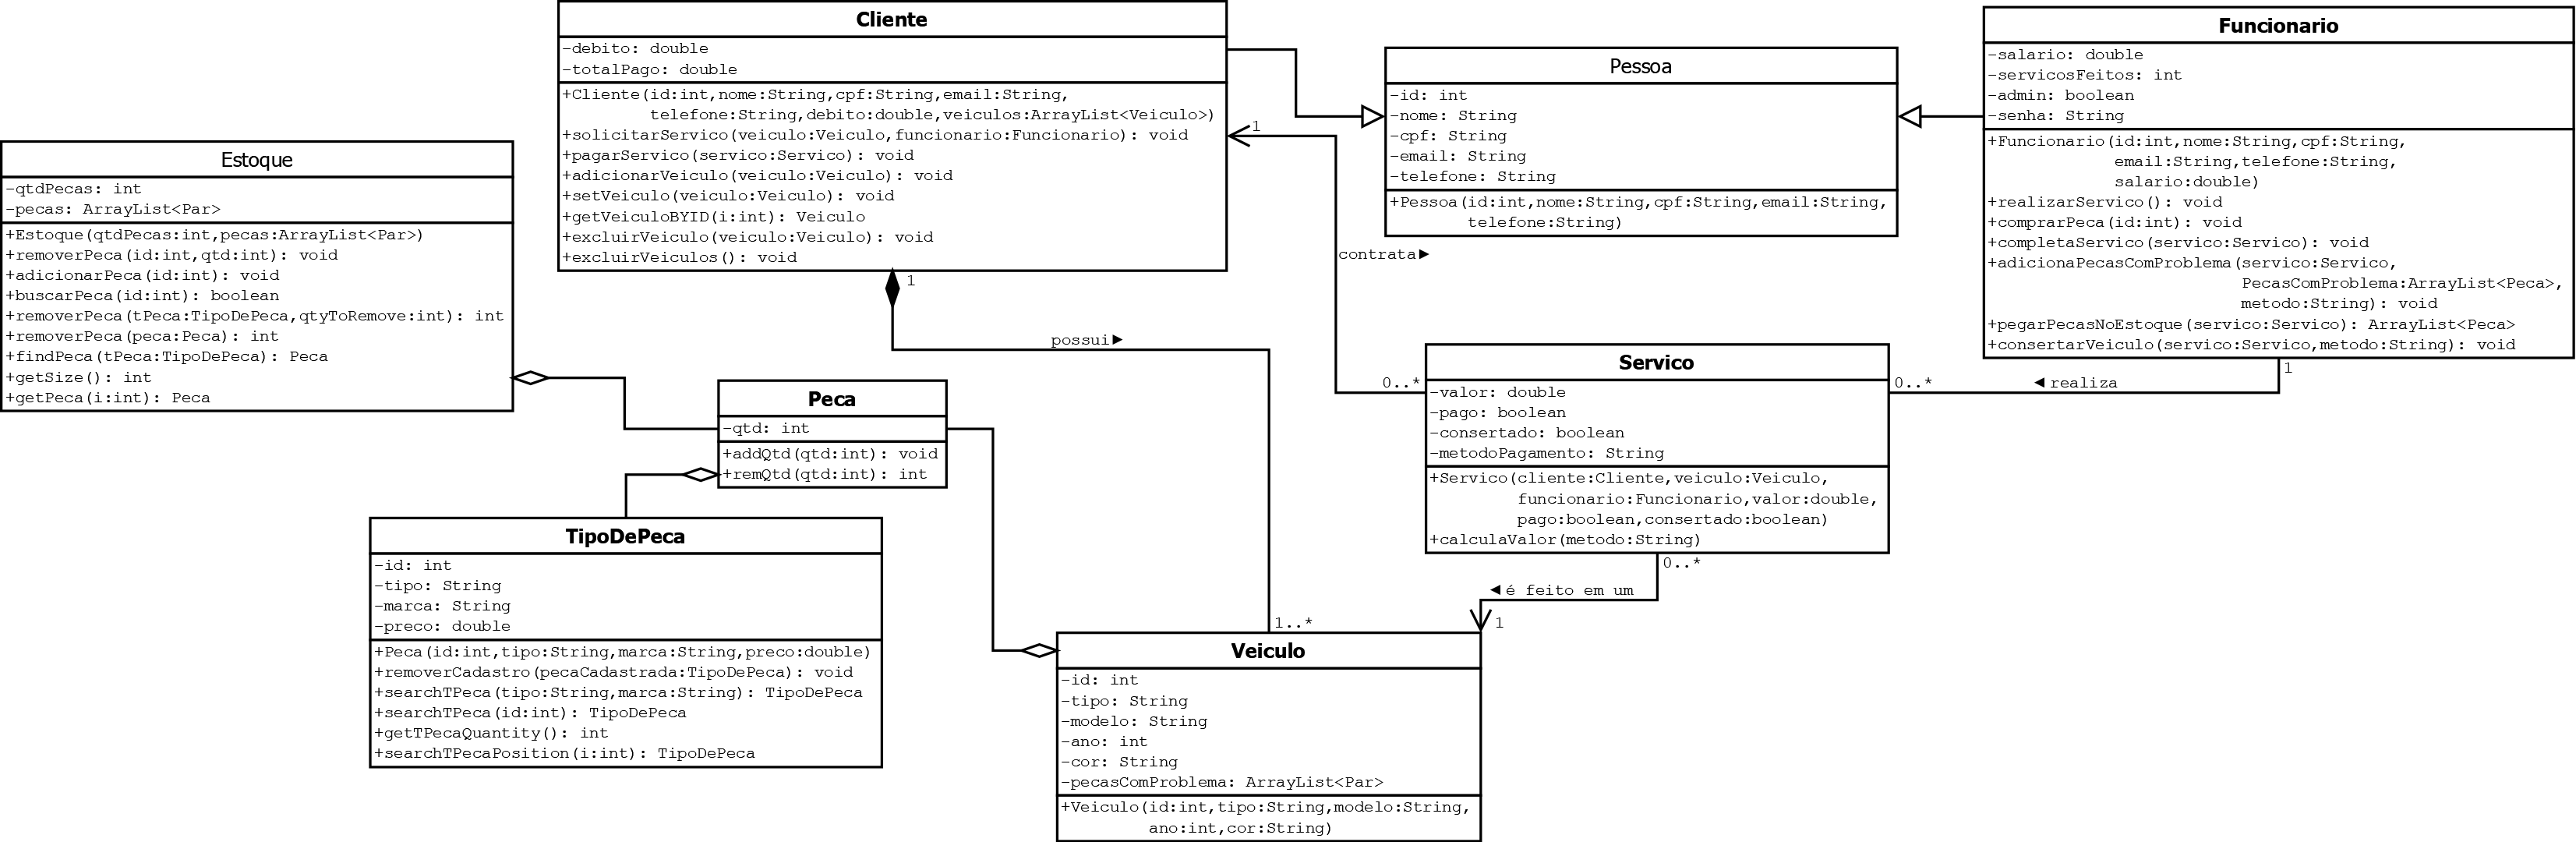
\includegraphics[width=\textwidth]{imagens/diagrama_de_classes.png}
    \caption{Diagrama de classes do sistema}
\end{figure}

\subsection{Classes do Sistema}

\subsubsection{TipoDePeça}
\paragraph{}
A classe \textit{TipoDePeça} fornece uma abstração para definir os tipos de peças reconhecidos e catalogados pela oficina. Ela possui um sistema de atribuição de códigos a cada novo tipo de peça cadastrado e permite busca por código ou pelos outros atributos: tipo e marca. Além disso, cada tipo de peça possui seu respectivo preço no catálogo. Todos os tipos de peças instanciados no programa são adicionados a uma lista estática da classe. Isso permite que as outras classes de fato usem \textit{TipoDePeça} da forma correta: nenhuma delas (fora a classe que implementa a tela de gerenciamento dos tipos de peça) instancia um novo tipo de peça: na verdade, elas utilizam referências a tipos de peça já existentes. Isso facilita inúmeras operações - ao invés de comparar se diversos atributos de uma peça são os mesmos de outra, por exemplo, podemos simplesmente verificar se é a mesma referência.

\paragraph{}
Essa classe possui os atributos descritos a seguir:

\begin{itemize}[noitemsep]
    \item \textbf{tPecasCadastradas} \textit{(static)}: Uma lista estática das peças conhecidas.
    \item \textbf{idGenerator} \textit{(static)}: Um atributo utilizado pela própria classe que ajuda a fornecer o serviço de geração de código das peças.
    \item \textbf{freeIds} \textit{(static)}: Uma lista que carrega códigos previamente utilizados, mas que foram liberados para uso futuro.
    \item \textbf{id}: O código da peça.
    \item \textbf{tipo}: O tipo da peça.
    \item \textbf{marca}: A marca da peça.
    \item \textbf{preco}: O preço da peça, um \textit{double}.
\end{itemize}

\noindent e os seguintes métodos (além dos getters e setters apropriados), que, com a exceção do construtor, são todos estáticos:
\begin{itemize}[noitemsep]
    \item \textbf{TipoDePeca()}: O construtor. Também executa toda a lógica de atribuição de código e reordena a lista.
    \item \textbf{removerCadastro()}: Remove o cadastro de um tipo de peça de acordo com uma referência ao objeto cadastrado.
    \item \textbf{searchTPeca()}: Um método com sobrecarga que permite pesquisar um tipo de peça na lista de acordo com seu código, ou tipo e marca.
    \item \textbf{getTPecaQuantity()}: Um getter especial que retorna a quantidade de peças cadastradas. Utilizado nas interfaces.
    \item \textbf{searchTPecaPosition()}: Um método de busca especial, também utilizado nas interfaces, que fornece uma forma de buscar uma peça pelo seu índice na lista.
\end{itemize}

\subsubsection{Peça}
\paragraph{}
A classe \textit{Peca} é uma classe muito simples, que "embrulha" duas informações: o \textit{TipoDePeca}, e a quantidade. Ela fornece uma abstração para representar as peças físicas. Ela possui os seguintes atributos:
\begin{itemize}[noitemsep]
    \item \textbf{tipoPeca}: O tipo da peça.
    \item \textbf{qtd}: A quantidade de peças.
\end{itemize}

\noindent além dos seguintes métodos:
\begin{itemize}[noitemsep]
    \item \textbf{Peca()}: O construtor padrão.
    \item \textbf{Peca(TipoDePeca tipoPeca, int qtd)}: O construtor que inicializa os atributos.
    \item \textbf{getTipoPeca()}: Retorna o tipo da peça.
    \item \textbf{getQtd()}: Retorna a quantidade de peças.
    \item \textbf{setQtd()}: Define a quantidade de peças.
    \item \textbf{addQtd()}: Adiciona uma quantidade de peças.
    \item \textbf{remQtd()}: Remove uma quantidade de peças.
\end{itemize}

\subsubsection{Estoque}
Estoque é uma classe abstrata pelo motivo de nunca ser instanciada (logo possui apenas membros estáticos), cuja função é autoexplicativa: é a representação do estoque da oficina. Ela possui um único atributo.

\begin{itemize}[noitemsep]
    \item \textbf{estoque}: Uma lista de peças.
\end{itemize}

\noindent Seus métodos, que proporcionam uma forma encapsulada de interação com essa lista, são os seguintes:

\begin{itemize}[noitemsep]
    \item \textbf{adicionarPeca()}: Um método que adiciona uma quantidade de uma peça ao estoque.
    \item \textbf{removerPeca()}: Um método sobrecarregado que pode remover uma determinade quantidade de uma peça do estoque utilizando um TipoDePeca e uma quantidade ou uma referência a um objeto Peca.
    \item \textbf{findPeca()}: Verifica se a peça está no estoque.
    \item \textbf{getSize()}: Retorna quantos tipos diferentes de peça há no estoque.
    \item \textbf{getPeca()}: Retorna a peça em um determinado índice da lista do estoque. 
\end{itemize}

\subsubsection{Veículo}
\paragraph{}
A classe \textit{Veiculo} modela os dados de um veículo. Uma lista dessas classes é um atributo da classe Cliente. Ela armazena as informações de id, ano, tipo, modelo, cor e placa, mas, principalmente, mantém uma lista de pecasComProblema, que é vazia até que o funcionário a popule pela tela de gerenciamento de serviços. A classe também oferece métodos para gerenciar os dados do veículo e manipular a lista de peças problemáticas, como adicionar peças com defeito e esvaziar a lista após os reparos. Essa estrutura permite uma organização eficiente dos diagnósticos e serviços realizados pela oficina.

\paragraph{}
A classe \textit{Veiculo} possui os seguintes atributos:
\begin{itemize}[noitemsep]
    \item \textbf{id}: O código do veículo.
    \item \textbf{ano}: O ano do veículo.
    \item \textbf{tipo}: O tipo do veículo.
    \item \textbf{modelo}: O modelo do veículo.
    \item \textbf{cor}: A cor do veículo.
    \item \textbf{placa}: A placa do veículo.
    \item \textbf{pecasComProblema}: Uma lista de peças com defeito.
\end{itemize}
\noindent e os seguintes métodos:
\begin{itemize}[noitemsep]
    \item \textbf{Veiculo()}: O construtor padrão.
    \item \textbf{Veiculo(int ano, String tipo, String placa, String modelo, String cor)}: O construtor que inicializa os atributos.
    \item \textbf{toString()}: Retorna a placa do veículo.
    \item \textbf{esvaziarPecasComProblema()}: Esvazia a lista de peças com defeito.
\end{itemize}

\subsubsection{Serviço}
\paragraph{}
A classe Serviços, por sua vez, é essencial para o sistema. Nela, quase todas as outras classes do projeto são instanciadas para que se realize o que esse sistema se propõe a fazer: permitir que se tenha controle sobre um reparo de um funcionário ao veículo de um cliente.

\paragraph{}
A classe \textit{Servico} possui os seguintes atributos:

\begin{itemize}[noitemsep]
    \item \textbf{id}: O código do serviço.
    \item \textbf{valor}: O valor do serviço.
    \item \textbf{pago}: Um booleano que indica se o serviço foi pago.
    \item \textbf{consertado}: Um booleano que indica se o veículo foi consertado.
    \item \textbf{metodoPagamento}: O método de pagamento.
    \item \textbf{cliente}: O cliente que solicitou o serviço.
    \item \textbf{veiculo}: O veículo que será consertado.
    \item \textbf{funcionario}: O funcionário que realizará o serviço.
\end{itemize}

\noindent e os seguintes métodos:

\begin{itemize}[noitemsep]
    \item \textbf{Servico()}: O construtor padrão.
    \item \textbf{Servico(Cliente cliente, Veiculo veiculo, Funcionario funcionario)}: O construtor que inicializa os atributos.
    \item \textbf{calculaValor()}: Calcula o valor do serviço.
    \item \textbf{adicionaPecasComProblema()}: Adiciona peças com defeito ao veículo.
\end{itemize}

\subsubsection{Pessoa}
\paragraph{}
A classe \textit{Pessoa} é uma classe abstrata que fornece a estrutura básica para representar pessoas no sistema. Ela é a superclasse de \textit{Cliente} e \textit{Funcionario}, que serão explicados doravante. A classe \textit{Pessoa} possui os seguintes atributos:

\begin{itemize}[noitemsep]
    \item \textbf{id}: O código da pessoa.
    \item \textbf{nome}: O nome da pessoa.
    \item \textbf{cpf}: O CPF da pessoa.
    \item \textbf{email}: O e-mail da pessoa.
    \item \textbf{telefone}: O telefone da pessoa.
\end{itemize}

\noindent e os seguintes métodos, além dos getters e setters:

\begin{itemize}[noitemsep]
    \item \textbf{Pessoa(int id, String nome, String cpf, String email, String telefone)}: O construtor que inicializa os atributos com id informado.
    \item \textbf{Pessoa(String nome, String cpf, String email, String telefone)}: O construtor que inicializa os atributos.
\end{itemize}

\subsubsection{Cliente}
\paragraph{}
A classe \textit{Cliente}, que herda a classe \textit{Pessoa}, oferece a estrutura para armazenar os dados de um cliente no contexto de uma oficina mecânica. Ela mantém informações como nome, telefone, endereço e uma lista de veículos associados ao cliente. Os objetos dessa classe são utilizados para criar os serviços da oficina. Os atributos dessa classe são os que seguem, além dos atributos herdados da classe \textit{Pessoa}:

\begin{itemize}[noitemsep]
    \item \textbf{debito}: O débito do cliente.
    \item \textbf{totalPago}: O total pago pelo cliente.
    \item \textbf{idGenerator}: atributo utilizado para criar o id do cliente quando ele é criado
    \item \textbf{idsLivres}: Uma lista dos ids livres para serem reutilizados
    \item \textbf{veiculos}: Uma lista de veículos associados ao cliente.
\end{itemize}

\noindent e os seguintes métodos, além dos getters e setters:

\begin{itemize}[noitemsep]
    \item \textbf{Cliente(String nome, String cpf, String email, String telefone)}: O construtor que inicializa os atributos.
    \item \textbf{excluirVeiculo(Veiculo veiculo)}: Exclui um veículo da lista de veículos.
    \item \textbf{excluirVeiculos()}: Exclui todos os veículos da lista de veículos.
\end{itemize}

\subsubsection{Funcionário}
\paragraph{}
A classe \textit{Funcionario}, que herda a classe \textit{Pessoa}, implementa uma estrutura para simular um funcionário no sistema da oficina. Ela fornece os métodos necessários para gerenciar os serviços e peças. Os atributos dessa classe são os que seguem, além dos atributos herdados da classe \textit{Pessoa}:

\begin{itemize}[noitemsep]
    \item \textbf{salario}: O salário do funcionário.
    \item \textbf{servicosFeitos}: A quantidade de serviços feitos pelo funcionário.
    \item \textbf{admin}: Um booleano que indica se o funcionário é administrador.
    \item \textbf{senha}: A senha do funcionário, utilizada para acessar o sistema.
    \item \textbf{servicosAtivos}: Um HashMap de serviços ativos, que mapeia o id do serviço ao serviço.
    \item \textbf{idsLivres}: Uma \textit{priority queue} dos ids livres para serem reutilizados.
    \item \textbf{idGenerator}: Um atributo utilizado para criar o id do funcionário quando ele é criado.
\end{itemize}

\noindent e os seguintes métodos, além dos getters e setters:

\begin{itemize}[noitemsep]
    \item \textbf{Funcionario(double salario, String senha, int id, String nome, String cpf, String email, String telefone)}: O construtor que inicializa os atributos com id informado.
    \item \textbf{Funcionario(double salario, String senha, String nome, String cpf, String email, String telefone)}: O construtor que inicializa os atributos.
    \item \textbf{Funcionario(String senha, String nome, String cpf, String email, String telefone)}: O construtor que inicializa os atributos sem salário informado.
    \item \textbf{completaServico(Servico servico)}: Completa um serviço.
    \item \textbf{pegarPecasNoEstoque(Servico servico)}: Gerencia as peças necessárias para um serviço, identificando as peças faltantes no estoque e removendo as peças disponíveis.
    \item \textbf{consertarVeiculo(Servico servico, String metodo)}: Calcula o valor de um serviço, esvazia a lista de peças com problema do veículo associado e define o serviço como consertado.
\end{itemize}

\subsection{Classes Auxiliares}

\subsubsection{Sessão de Usuário}
\paragraph{}
A classe \textit{SessaoUsuario} é uma classe auxiliar que fornece ao sistema uma lógica de sessão do usuário autenticado no momento. Ela mantém uma referência estática ao funcionário logado, que é criada quando o usuário faz a autenticação pela tela de Login. Os atributos dessa classe são os que seguem:

\begin{itemize}[noitemsep]
    \item \textbf{instancia}: Inicializa a única instância do usuário logado.
    \item \textbf{usuarioLogado}: O funcionário logado.
\end{itemize}

\noindent e os métodos são os seguintes:

\begin{itemize}[noitemsep]
    \item \textbf{SessaoUsuario()}: O construtor \textbf{privado}, para impedir a criação de múltiplas instâncias.
    \item \textbf{getInstancia()}: Retorna a instância do usuário logado.
    \item \textbf{setUsuarioLogado(Funcionario usuarioLogado)}: Define o funcionário logado.
    \item \textbf{getUsuarioLogado()}: Retorna o funcionário logado.
\end{itemize}

\paragraph{}
Para essa classe, forceremos a implementação por aqui, para que ela seja melhor compreendida.

\begin{code}
\begin{minted}[breaklines=true, breakanywhere=true, linenos=true, bgcolor=cinza_claro, style=manni]{java}
package app.utils;

import app.model.Funcionario;

public class SessaoUsuario {
    private static SessaoUsuario instancia;
    private Funcionario usuarioLogado;

    private SessaoUsuario() {}

    public static SessaoUsuario getInstancia() {
        if (instancia == null) {
            instancia = new SessaoUsuario();
        }
        return instancia;
    }

    public void setUsuarioLogado(Funcionario usuario) {
        this.usuarioLogado = usuario;
    }

    public Funcionario getUsuarioLogado() {
        return usuarioLogado;
    }
}
\end{minted}
\caption{Implementação da classe SessaoUsuario}
\end{code}

\subsubsection{idGenerator}
\paragraph{}
Essa classe foi utilizada por algumas classes para gerar códigos únicos para os objetos. Ela fornece um método estático que retorna um código único para cada objeto criado. O código é gerado a partir de um contador que é incrementado a cada chamada do método. A classe possui os seguintes atributos estáticos:

\begin{itemize}[noitemsep]
    \item \textbf{currentServicoId}: O contador dos ids de serviços.
    \item \textbf{currentVeiculoId}: O contador dos ids de veículos.
\end{itemize}

\noindent e os seguintes métodos:

\begin{itemize}[noitemsep]
    \item \textbf{generateServicoID()}: Gera um id único para um serviço.
    \item \textbf{generateVeiculoID()}: Gera um id único para um veículo.
\end{itemize}

\noindent Ambos \textit{synchronized}, isto é, que podem ser acessados apenas por uma thread por vez, para evitar problemas de concorrência.

\subsubsection{Objetos}
\paragraph{}
A classe \textit{Objetos} é uma classe auxiliar que mantém \textit{HashMap}s públicos e estáticos de todas as classes do sistema, armazenando os objetos criados de cada classe na interface de forma a simular o funcionamento real de um sistema com persistência durante a execução do programa. Além disso, nessa classe são criados, na execução do programa, os objetos padrão de cada classe, de forma a facilitar a visualização e o teste do sistema. Os atributos dessa classe são os que seguem:

\begin{itemize}[noitemsep]
    \item \textbf{clientes}: Um \textit{HashMap} de clientes.
    \item \textbf{funcionarios}: Um \textit{HashMap} de funcionários.
    \item \textbf{veiculos}: Um \textit{HashMap} de veículos.
    \item \textbf{servicos}: Um \textit{HashMap} de serviços.
    \item \textbf{placas}: Uma \textit{ArrayList} de placas de veículos.
\end{itemize}

\noindent seus métodos são demasiados e uma descrição detalhada para cada um deles não é necessária, mas, em resumo, eles são responsáveis por criar os objetos de exemplo no sistema.

% Telas
\section{Telas}

\subsection{Telas de Início}
\begin{figure}[H]
    \centering
    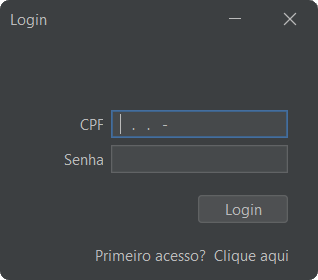
\includegraphics[width=0.5\linewidth]{imagens/telaLogin.png}
    \caption{Tela de login}
\end{figure}

\begin{figure}[H]
    \centering
    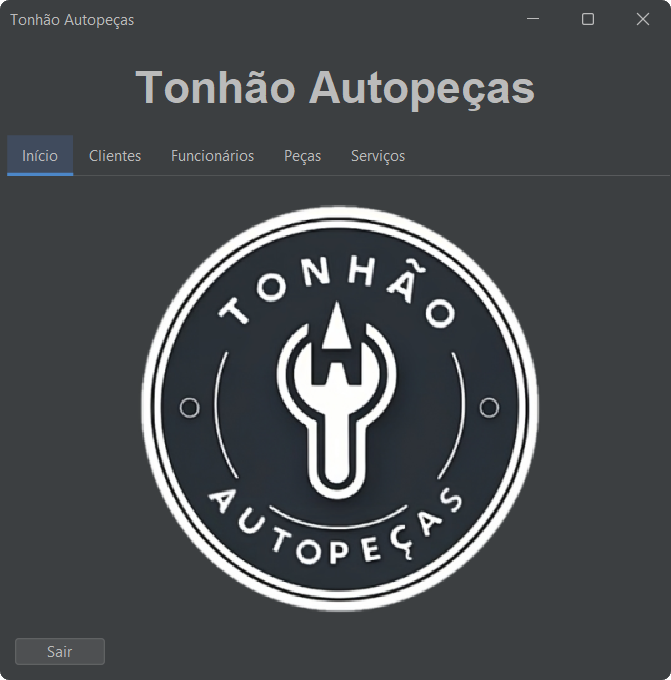
\includegraphics[width=0.5\linewidth]{imagens/telaInicial.png}
    \caption{Tela inicial}
\end{figure}

\begin{figure}[H]
    \centering
    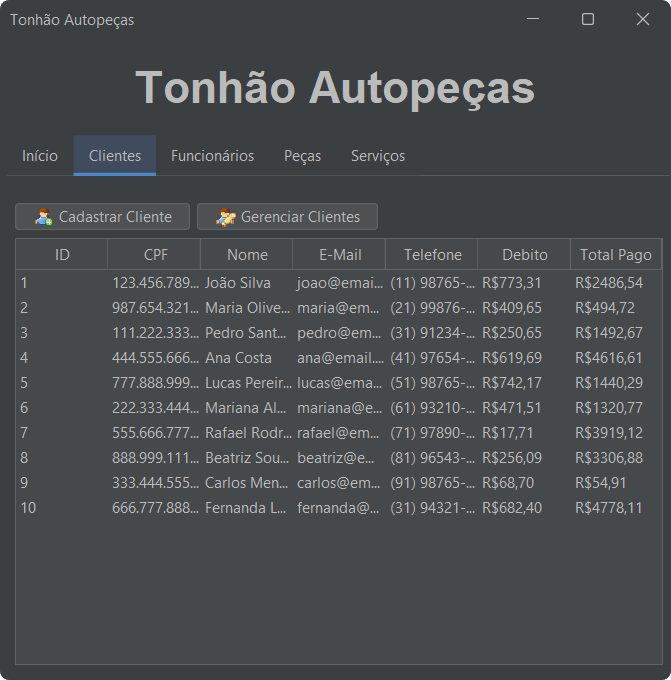
\includegraphics[width=0.5\linewidth]{imagens/telaInicioClientes.png}
    \caption{Tela inicial - Seção de clientes}
\end{figure}

\begin{figure}[H]
    \centering
    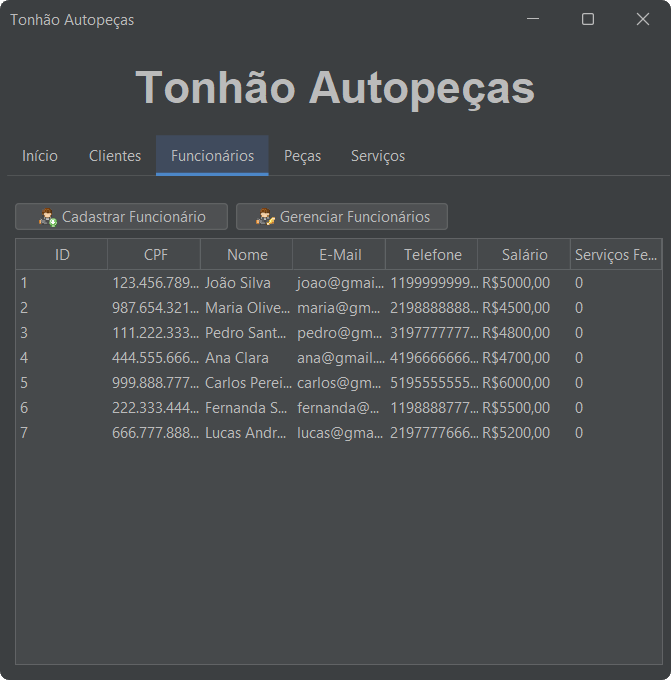
\includegraphics[width=0.5\linewidth]{imagens/telaInicioFuncionarios.png}
    \caption{Tela inicial - Seção de funcionários}
\end{figure}

\begin{figure}[H]
    \centering
    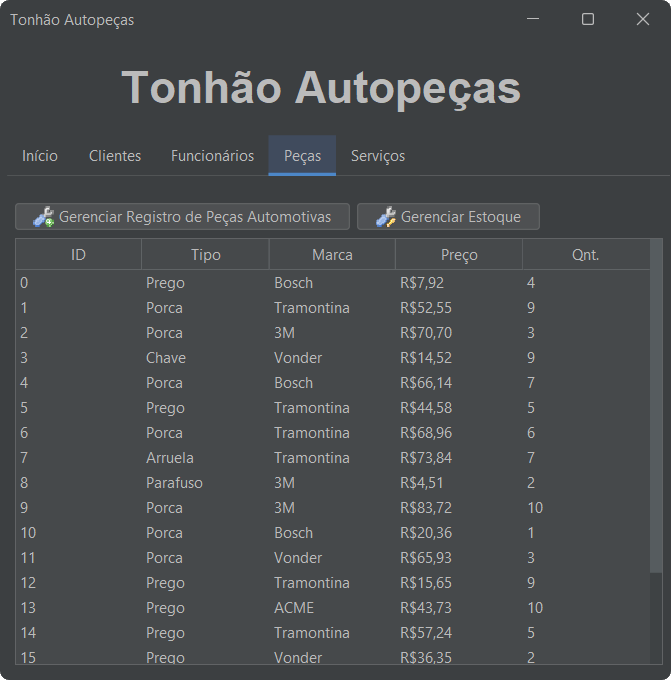
\includegraphics[width=0.5\linewidth]{imagens/telaInicioPecas.png}
    \caption{Tela inicial - Seção de peças}
\end{figure}

\begin{figure}[H]
    \centering
    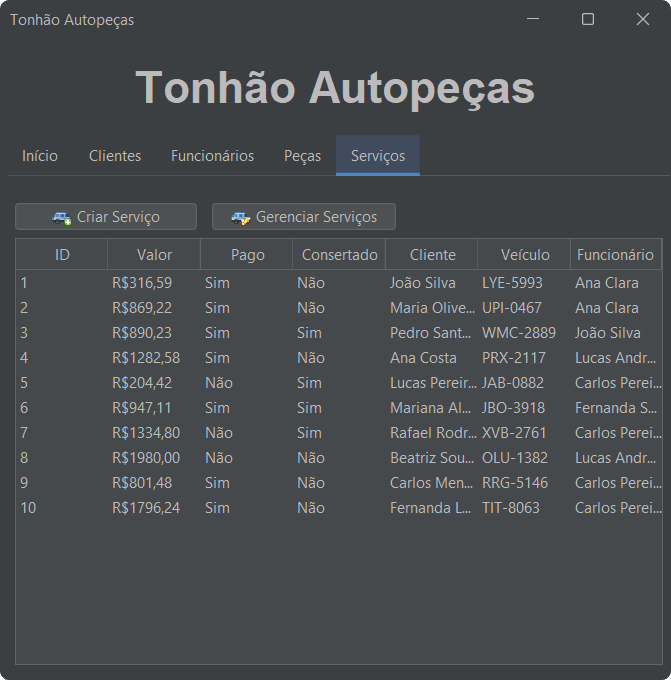
\includegraphics[width=0.5\linewidth]{imagens/telaInicioServicos.png}
    \caption{Tela inicial - Seção de serviços}
\end{figure}

\subsection{Telas de Cadastro e Criação}

\begin{figure}[H]
    \centering
    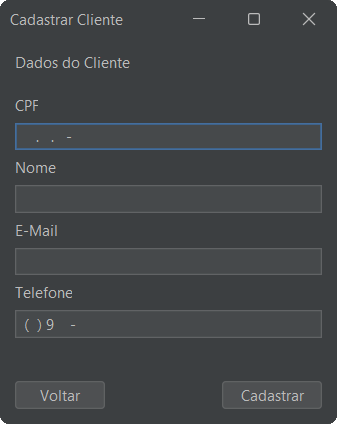
\includegraphics[width=0.5\linewidth]{imagens/cadastroClientes.png}
    \caption{Tela de Cadastro - Clientes}
\end{figure}

\begin{figure}[H]
    \centering
    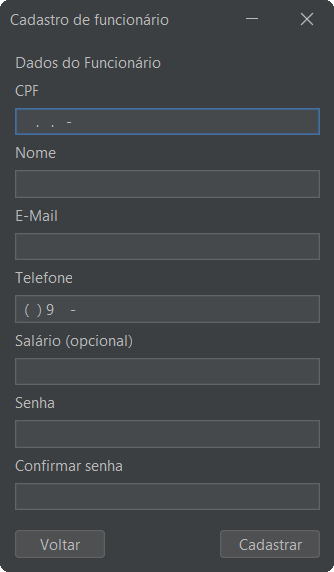
\includegraphics[width=0.5\linewidth]{imagens/cadastroFuncionarios.png}
    \caption{Tela de Cadastro - Funcionários}
\end{figure}

\begin{figure}[H]
    \centering
    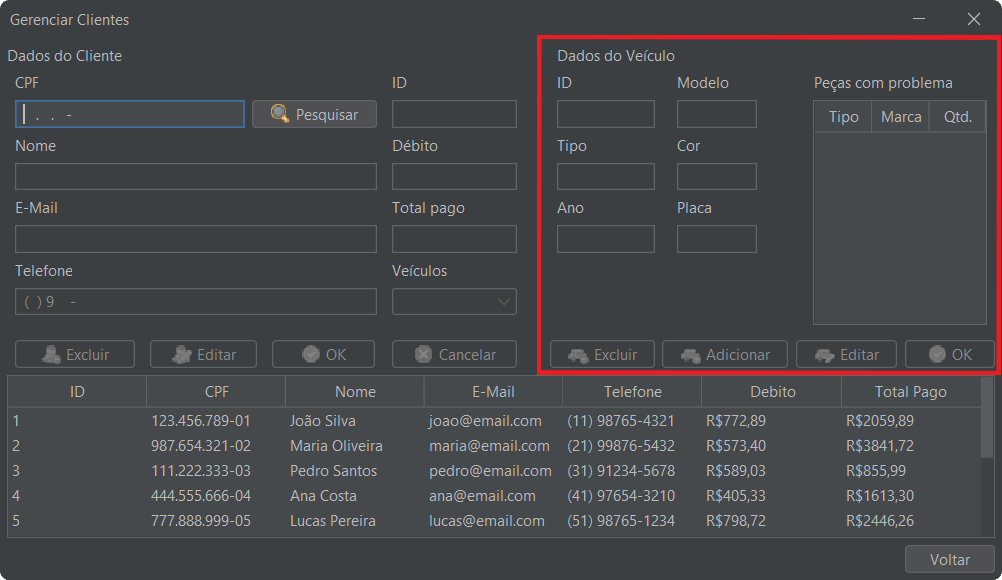
\includegraphics[width=0.75\linewidth]{imagens/cadastroVeiculos.png}
    \caption{Tela de Cadastro - Veículos}
\end{figure}

\begin{figure}[H]
    \centering
    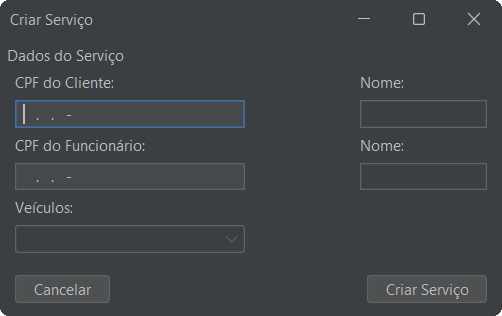
\includegraphics[width=0.5\linewidth]{imagens/criarServico.png}
    \caption{Tela de Criação de Serviços}
\end{figure}


\subsection{Telas de Gerenciamento}

\begin{figure}[H]
    \centering
    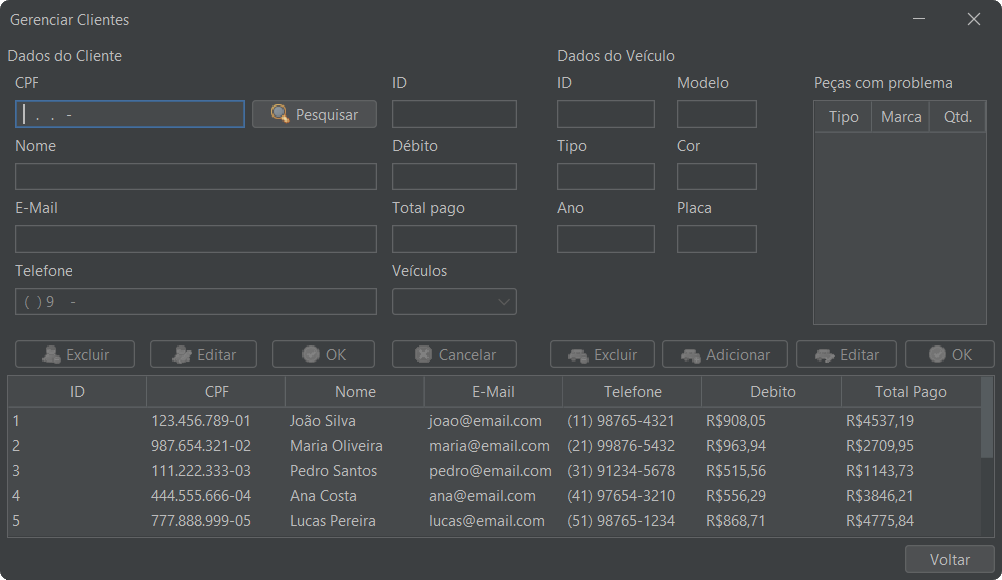
\includegraphics[width=0.75\linewidth]{imagens/gerenciarClientes.png}
    \caption{Tela de gerência de clientes}
\end{figure}

\begin{figure}[H]
    \centering
    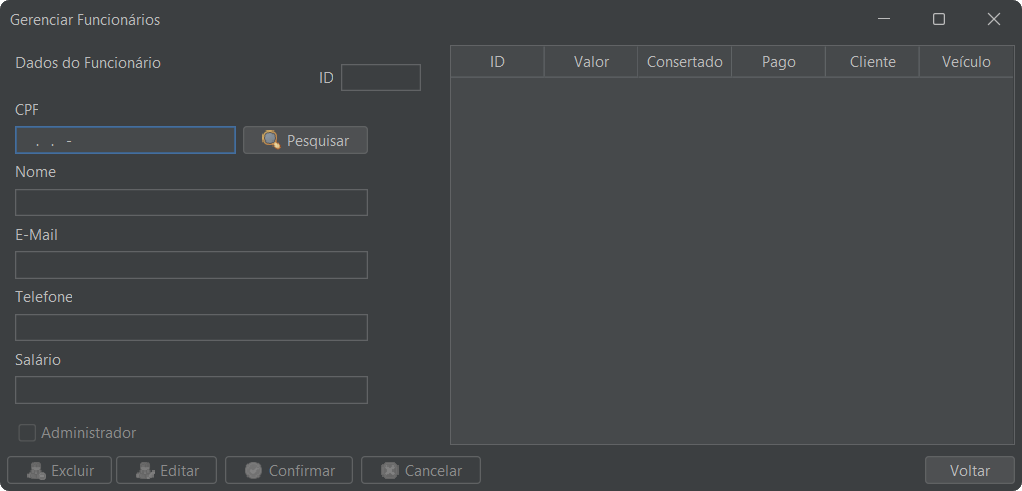
\includegraphics[width=0.75\linewidth]{imagens/gerenciarFuncionarios.png}
    \caption{Tela de gerência de funcionários}
\end{figure}

\begin{figure}[H]
    \centering
    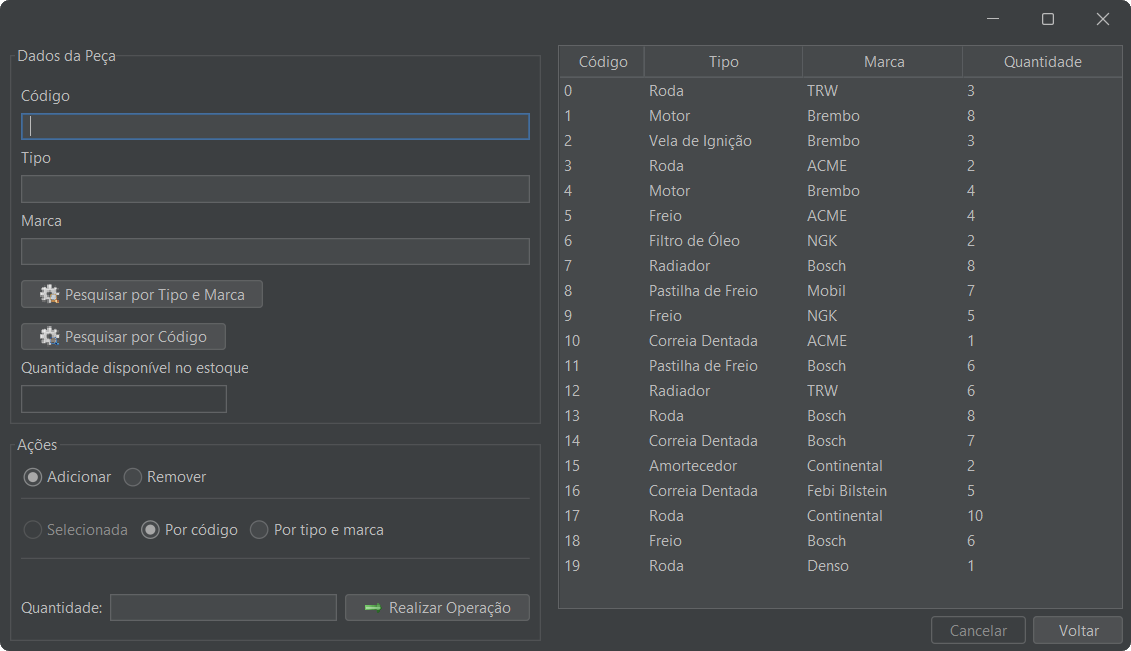
\includegraphics[width=0.75\linewidth]{imagens/gerenciarEstoque.png}
    \caption{Tela de gerência do estoque}
\end{figure}

\begin{figure}[H]
    \centering
    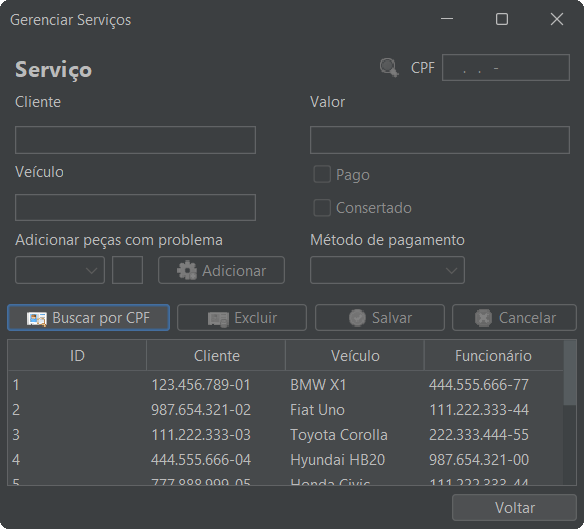
\includegraphics[width=0.75\linewidth]{imagens/gerenciarServicos.png}
    \caption{Tela de gerência de serviços}
\end{figure}

\end{document}